\documentclass{article}
\usepackage[utf8]{inputenc}
\usepackage{amsmath}
\usepackage{graphicx}
\graphicspath{ {images/} }

\title{Alberi binari di ricerca e alberi rosso-neri a confronto}
\author{Marco Benelli}
\date{Settembre 2019}

\begin{document}

\maketitle

\section{Introduzione}

L'obiettivo è confrontare le velocità e le complessità della ricerca di elementi in due strutture dati e verificare che queste siano coerenti con i risultati teorici.

\section{Teoria}

\subsection{Albero binario di ricerca}

Dallo studio teorico sappiamo che l'albero binario di ricerca ha un'altezza media logaritmica rispetto al numero di elementi totale ($\Theta(\log(n)$). Però sappiamo anche che nel caso peggiore ha un'altezza lineare ($\Theta(n)$).

\subsection{Albero rosso nero}

L'albero rosso nero ha sempre (anche nel caso peggiore) un'altezza logaritmica ($\Theta(\log(n))$).

\section{Prestazioni attese}

Le complessità di cui si è parlato nella sezione precedente sono da intendersi come asintotiche. I tempi di esecuzione possono avere un andamento diverso per alberi piccoli. Quello che speriamo è che raggiungano un andamento simile a quello teorico anche per alberi relativamente piccoli.

\section{Esperimenti}

Verranno svolti 4 esperimenti: 2 per l'albero binario di ricerca e 2 per l'albero rosso nero, 2 facendo inserimenti casuali e 2 inserendo gli elementi in ordine. Gli esperimenti verranno condotti su alberi di grandezza sempre crescente (ogni volta la grandezza viene raddoppiata) finché il tempo di esecuzione non supera i 128 secondi. Nel caso di inserimenti casuali, per ogni grandezza e per ogni classe di albero vengono condotti 8 test; mentre per inserimenti ordinati si farà un solo test.

Anziché calcolare direttamente i tempi di esecuzione delle ricerche, verrà calcolata l'altezza degli alberi. È importante notare che, anche nel caso di inserimenti casuali, in entrambe le classi di alberi verranno inseriti gli stessi numeri, in modo da avere una valutazione più equa.

\section{Codice}

Il codice è diviso in quattro sezioni: le classi e i metodi che implementano gli alberi (queste sono semplicemente delle traduzioni in Python dello pseudo codice visto a lezione), le funzioni per la creazione degli alberi, le funzioni che implementano i test e le funzioni che disegnano i grafici.

Le funzioni per la generazione usano il comando yield per non dover creare una lista e occupare troppa memoria e la funzione random della libreria standard.

Per misurare le altezze degli alberi viene usata una funzione ricorsiva che che visita tutti i nodi che nel codice viene chiamata get\_height.

Per quanto riguarda i grafici, si usa la libreria matplotlib, nello specifico il modulo pyplot. I vettori che vengono dati alla funzione plot sono il vettore delle grandezze degli alberi (come vettore delle ascisse) e il vettore delle altezze (come vettore delle ordinate) per ogni test. Oltre a queste quattro curve (separate in due figure), vengono anche disegnate altre quattro curve che simboleggiano l'andamento predetto dalla teoria per confrontarlo con l'andamento sperimentale.

\section{Risultati sperimentali}

\begin{figure}[ht]
    \centering
    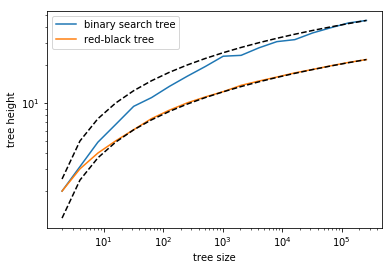
\includegraphics{random}
    \caption{Il grafico del test con inserimenti casuali. Possiamo osservare che il grafico dell'albero binario di ricerca è più "casuale" proprio perché non avviene alcun tipo di bilanciamento.}
    \label{fig:random}
\end{figure}

\begin{figure}[ht]
    \centering
    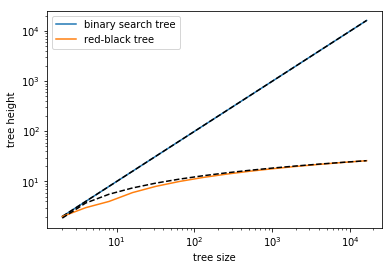
\includegraphics{sorted}
    \caption{Il grafico del test con inserimenti ordinati. L'albero binario di ricerca ha un'altezza lineare, mentre l'albero rosso-nero ha un'altezza logaritmica.}
    \label{fig:sorted}
\end{figure}

Nelle figure \ref{fig:random} e \ref{fig:sorted} possiamo vedere che i risultati sperimentali sono in linea con le predizioni teoriche visto che le linee colorate si sovrappongono a quelle tratteggiate. È importante notare che i grafici sono in scala logaritmica, in modo che complessità lineari possano essere rappresentate con una retta. Le linee tratteggiate indicano l'andamento teorico e sono ottenute moltiplicando la funzione teorica per un coefficiente opportuno. Questo coefficiente si trova imponendo che la linea tratteggiata e quella colorata abbiano in comune l'ultimo punto.

Questi risultati ci fanno concludere che l'albero rosso-nero è sempre migliore dell'albero binario di ricerca e quest'ultimo si può usare solo nel caso di alberi molto piccoli.

\end{document}
